\documentclass{article}\usepackage[]{graphicx}\usepackage[]{color}
%% maxwidth is the original width if it is less than linewidth
%% otherwise use linewidth (to make sure the graphics do not exceed the margin)
\makeatletter
\def\maxwidth{ %
  \ifdim\Gin@nat@width>\linewidth
    \linewidth
  \else
    \Gin@nat@width
  \fi
}
\makeatother

\definecolor{fgcolor}{rgb}{0.345, 0.345, 0.345}
\newcommand{\hlnum}[1]{\textcolor[rgb]{0.686,0.059,0.569}{#1}}%
\newcommand{\hlstr}[1]{\textcolor[rgb]{0.192,0.494,0.8}{#1}}%
\newcommand{\hlcom}[1]{\textcolor[rgb]{0.678,0.584,0.686}{\textit{#1}}}%
\newcommand{\hlopt}[1]{\textcolor[rgb]{0,0,0}{#1}}%
\newcommand{\hlstd}[1]{\textcolor[rgb]{0.345,0.345,0.345}{#1}}%
\newcommand{\hlkwa}[1]{\textcolor[rgb]{0.161,0.373,0.58}{\textbf{#1}}}%
\newcommand{\hlkwb}[1]{\textcolor[rgb]{0.69,0.353,0.396}{#1}}%
\newcommand{\hlkwc}[1]{\textcolor[rgb]{0.333,0.667,0.333}{#1}}%
\newcommand{\hlkwd}[1]{\textcolor[rgb]{0.737,0.353,0.396}{\textbf{#1}}}%

\usepackage{framed}
\makeatletter
\newenvironment{kframe}{%
 \def\at@end@of@kframe{}%
 \ifinner\ifhmode%
  \def\at@end@of@kframe{\end{minipage}}%
  \begin{minipage}{\columnwidth}%
 \fi\fi%
 \def\FrameCommand##1{\hskip\@totalleftmargin \hskip-\fboxsep
 \colorbox{shadecolor}{##1}\hskip-\fboxsep
     % There is no \\@totalrightmargin, so:
     \hskip-\linewidth \hskip-\@totalleftmargin \hskip\columnwidth}%
 \MakeFramed {\advance\hsize-\width
   \@totalleftmargin\z@ \linewidth\hsize
   \@setminipage}}%
 {\par\unskip\endMakeFramed%
 \at@end@of@kframe}
\makeatother

\definecolor{shadecolor}{rgb}{.97, .97, .97}
\definecolor{messagecolor}{rgb}{0, 0, 0}
\definecolor{warningcolor}{rgb}{1, 0, 1}
\definecolor{errorcolor}{rgb}{1, 0, 0}
\newenvironment{knitrout}{}{} % an empty environment to be redefined in TeX

\usepackage{alltt}
\usepackage[sc]{mathpazo}
\renewcommand{\sfdefault}{lmss}
\renewcommand{\ttdefault}{lmtt}
\usepackage[T1]{fontenc}
\usepackage{geometry}
\geometry{verbose,tmargin=2.5cm,bmargin=2.5cm,lmargin=2.5cm,rmargin=2.5cm}
\setcounter{secnumdepth}{2}
\setcounter{tocdepth}{2}
\usepackage[unicode=true,pdfusetitle,
 bookmarks=true,bookmarksnumbered=true,bookmarksopen=true,bookmarksopenlevel=2,
 breaklinks=false,pdfborder={0 0 1},backref=false,colorlinks=false]
 {hyperref}
\hypersetup{
 pdfstartview={XYZ null null 1}}

\makeatletter
%%%%%%%%%%%%%%%%%%%%%%%%%%%%%% User specified LaTeX commands.
\renewcommand{\textfraction}{0.05}
\renewcommand{\topfraction}{0.8}
\renewcommand{\bottomfraction}{0.8}
\renewcommand{\floatpagefraction}{0.75}

\makeatother
\IfFileExists{upquote.sty}{\usepackage{upquote}}{}
\begin{document}








The results below are generated from an R script.


\begin{knitrout}
\definecolor{shadecolor}{rgb}{0.969, 0.969, 0.969}\color{fgcolor}\begin{kframe}
\begin{alltt}
\hlstd{cubic_fit} \hlkwb{<-} \hlkwd{lm}\hlstd{(nox} \hlopt{~} \hlkwd{poly}\hlstd{(dis,} \hlnum{3}\hlstd{),} \hlkwc{data} \hlstd{= Boston)}
\hlkwd{coef}\hlstd{(}\hlkwd{summary}\hlstd{(cubic_fit))}
\end{alltt}
\begin{verbatim}
##               Estimate Std. Error t value   Pr(>|t|)
## (Intercept)     0.5547   0.002759 201.021  0.000e+00
## poly(dis, 3)1  -2.0031   0.062071 -32.271 1.597e-124
## poly(dis, 3)2   0.8563   0.062071  13.796  6.133e-37
## poly(dis, 3)3  -0.3180   0.062071  -5.124  4.275e-07
\end{verbatim}
\begin{alltt}
\hlstd{dislims} \hlkwb{<-} \hlkwd{range}\hlstd{(dis)}
\hlstd{dis_grid} \hlkwb{<-} \hlkwd{seq}\hlstd{(}\hlkwc{from} \hlstd{= dislims[}\hlnum{1}\hlstd{],} \hlkwc{to} \hlstd{= dislims[}\hlnum{2}\hlstd{])}
\hlstd{cubic_pred} \hlkwb{<-} \hlkwd{predict}\hlstd{(cubic_fit,} \hlkwc{newdata} \hlstd{=} \hlkwd{list}\hlstd{(}\hlkwc{dis} \hlstd{= dis_grid),} \hlkwc{se} \hlstd{=} \hlnum{TRUE}\hlstd{)}
\hlstd{se_bands} \hlkwb{<-} \hlkwd{cbind}\hlstd{(cubic_pred}\hlopt{$}\hlstd{fit} \hlopt{+} \hlnum{2}\hlopt{*}\hlstd{cubic_pred}\hlopt{$}\hlstd{se.fit,}
                  \hlstd{cubic_pred}\hlopt{$}\hlstd{fit} \hlopt{-} \hlnum{2}\hlopt{*}\hlstd{cubic_pred}\hlopt{$}\hlstd{se.fit)}
\hlkwd{par}\hlstd{(}\hlkwc{mar} \hlstd{=} \hlkwd{c}\hlstd{(}\hlnum{4.5}\hlstd{,}\hlnum{4.5}\hlstd{,}\hlnum{1}\hlstd{,}\hlnum{1}\hlstd{),} \hlkwc{oma} \hlstd{=} \hlkwd{c}\hlstd{(}\hlnum{0}\hlstd{,}\hlnum{0}\hlstd{,}\hlnum{2}\hlstd{,}\hlnum{0}\hlstd{))}
\hlkwd{plot}\hlstd{(dis, nox,} \hlkwc{xlim} \hlstd{= dislims,} \hlkwc{col} \hlstd{=} \hlstr{"darkgrey"}\hlstd{,} \hlkwc{xlab} \hlstd{=} \hlstr{"dis"}\hlstd{,} \hlkwc{ylab} \hlstd{=} \hlstr{"nox"}\hlstd{)}
\hlkwd{title}\hlstd{(}\hlstr{"Cubic Polynomial"}\hlstd{,} \hlkwc{outer} \hlstd{=} \hlnum{FALSE}\hlstd{)} \hlcom{# title that spans both plots}
\hlkwd{lines}\hlstd{(dis_grid, cubic_pred}\hlopt{$}\hlstd{fit,} \hlkwc{lwd} \hlstd{=} \hlnum{2}\hlstd{,} \hlkwc{col} \hlstd{=} \hlstr{"red"}\hlstd{)}
\hlkwd{matlines}\hlstd{(dis_grid, se_bands,} \hlkwc{lwd} \hlstd{=} \hlnum{3}\hlstd{,} \hlkwc{col} \hlstd{=} \hlstr{"orange"}\hlstd{,} \hlkwc{lty} \hlstd{=} \hlnum{3}\hlstd{)}
\end{alltt}
\end{kframe}

{\centering 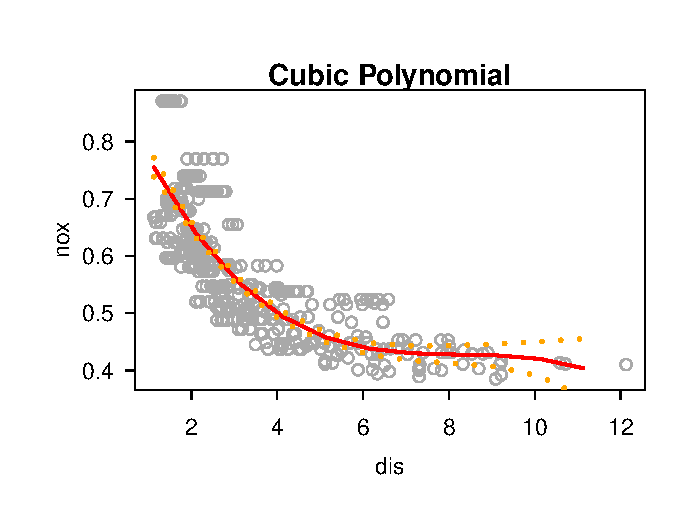
\includegraphics[width=.6\linewidth]{figure/Schmidt-HW7-Rnwunnamed-chunk-2-1} 

}



\end{knitrout}
\begin{knitrout}
\definecolor{shadecolor}{rgb}{0.969, 0.969, 0.969}\color{fgcolor}

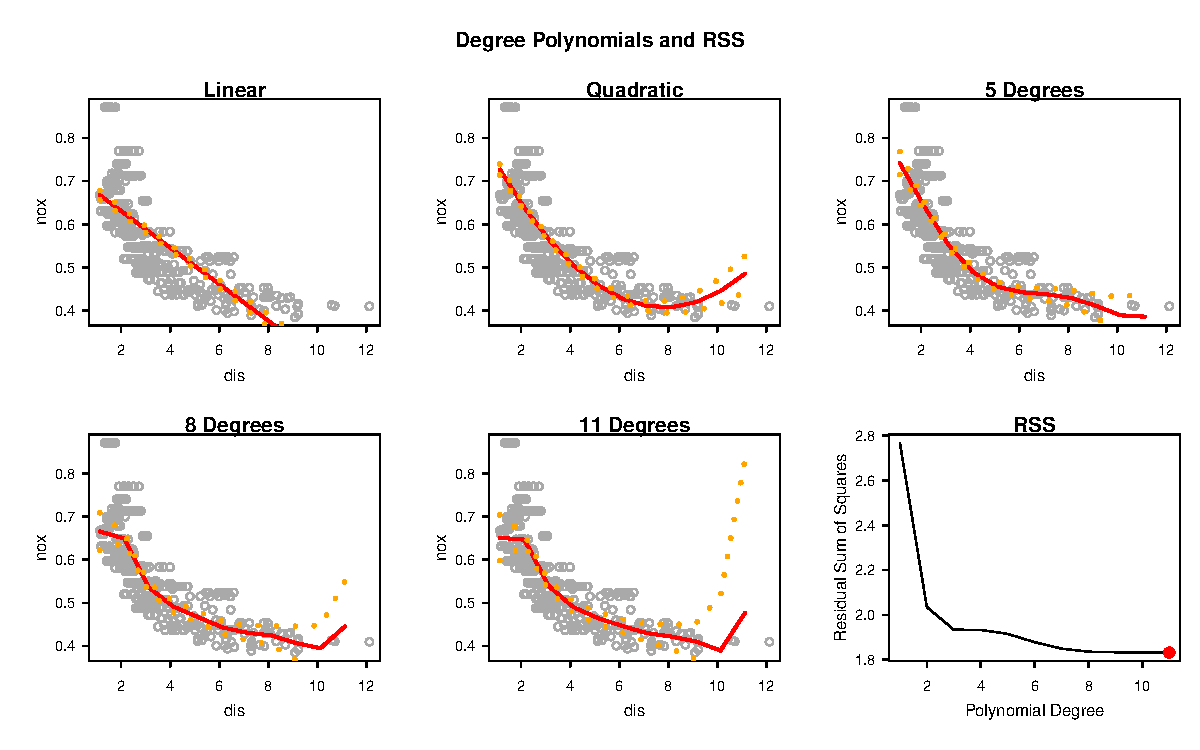
\includegraphics[width=.6\linewidth]{figure/Schmidt-HW7-Rnwunnamed-chunk-3-1} \hfill{}



\end{knitrout}
\begin{knitrout}
\definecolor{shadecolor}{rgb}{0.969, 0.969, 0.969}\color{fgcolor}\begin{kframe}
\begin{alltt}
\hlstd{prediction_error} \hlkwb{<-} \hlkwd{rep}\hlstd{(}\hlnum{0}\hlstd{,} \hlnum{10}\hlstd{)}
\hlkwa{for} \hlstd{(i} \hlkwa{in} \hlnum{1}\hlopt{:}\hlnum{10}\hlstd{)\{} \hlcom{# Run all the polynomial models and store them}
  \hlcom{# Use the glm function for poly models instead of lm so we can use cv.glm}
   \hlstd{poly_fit} \hlkwb{<-} \hlkwd{glm}\hlstd{(nox} \hlopt{~} \hlkwd{poly}\hlstd{(dis, i),} \hlkwc{data} \hlstd{= Boston)}
   \hlstd{prediction_error[i]} \hlkwb{<-} \hlkwd{cv.glm}\hlstd{(Boston, poly_fit,} \hlkwc{K} \hlstd{=} \hlnum{10}\hlstd{)}\hlopt{$}\hlstd{delta[}\hlnum{1}\hlstd{]\}}
\hlkwd{par}\hlstd{(}\hlkwc{mfrow} \hlstd{=} \hlkwd{c}\hlstd{(}\hlnum{1}\hlstd{,}\hlnum{1}\hlstd{),}  \hlkwc{mar} \hlstd{=} \hlkwd{c}\hlstd{(}\hlnum{4.5}\hlstd{,}\hlnum{4.5}\hlstd{,}\hlnum{1}\hlstd{,}\hlnum{1}\hlstd{),} \hlkwc{oma} \hlstd{=} \hlkwd{c}\hlstd{(}\hlnum{0}\hlstd{,}\hlnum{0}\hlstd{,}\hlnum{2}\hlstd{,}\hlnum{0}\hlstd{))} \hlcom{# plot it!}
\hlkwd{plot}\hlstd{(}\hlnum{1}\hlopt{:}\hlnum{10}\hlstd{, prediction_error,} \hlkwc{xlab} \hlstd{=} \hlstr{"Degree"}\hlstd{,} \hlkwc{ylab} \hlstd{=} \hlstr{"CV Error"}\hlstd{,} \hlkwc{type} \hlstd{=} \hlstr{"l"}\hlstd{)}
\hlstd{d.min} \hlkwb{<-} \hlkwd{which.min}\hlstd{(prediction_error)}
\hlkwd{points}\hlstd{(}\hlkwd{which.min}\hlstd{(prediction_error), prediction_error[}\hlkwd{which.min}\hlstd{(prediction_error)],}
       \hlkwc{col} \hlstd{=} \hlstr{"red"}\hlstd{,} \hlkwc{cex} \hlstd{=} \hlnum{2}\hlstd{,} \hlkwc{pch} \hlstd{=} \hlnum{20}\hlstd{)}
\end{alltt}
\end{kframe}

{\centering 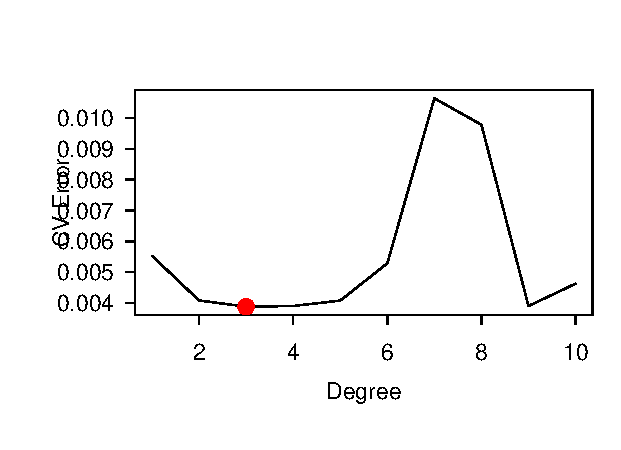
\includegraphics[width=.6\linewidth]{figure/Schmidt-HW7-Rnwunnamed-chunk-4-1} 

}



\end{knitrout}
\begin{knitrout}
\definecolor{shadecolor}{rgb}{0.969, 0.969, 0.969}\color{fgcolor}\begin{kframe}
\begin{alltt}
\hlstd{spline_fit} \hlkwb{<-} \hlkwd{lm}\hlstd{(nox} \hlopt{~} \hlkwd{bs}\hlstd{(dis,} \hlkwc{df} \hlstd{=} \hlnum{4}\hlstd{),} \hlkwc{data} \hlstd{= Wage)}
\hlstd{spline_pred} \hlkwb{<-} \hlkwd{predict}\hlstd{(spline_fit,} \hlkwc{newdata} \hlstd{=} \hlkwd{list}\hlstd{(}\hlkwc{dis} \hlstd{= dis_grid),} \hlkwc{se} \hlstd{=} \hlnum{TRUE}\hlstd{)}
\hlkwd{par}\hlstd{(}\hlkwc{mar} \hlstd{=} \hlkwd{c}\hlstd{(}\hlnum{4.5}\hlstd{,}\hlnum{4.5}\hlstd{,}\hlnum{1}\hlstd{,}\hlnum{1}\hlstd{),} \hlkwc{oma} \hlstd{=} \hlkwd{c}\hlstd{(}\hlnum{0}\hlstd{,}\hlnum{0}\hlstd{,}\hlnum{2}\hlstd{,}\hlnum{0}\hlstd{))}
\hlkwd{plot}\hlstd{(dis, nox,} \hlkwc{col} \hlstd{=} \hlstr{"gray"}\hlstd{);}\hlkwd{title}\hlstd{(}\hlstr{"Quartic"}\hlstd{,} \hlkwc{outer} \hlstd{=} \hlnum{FALSE}\hlstd{)}  \hlcom{# Plot the output}
\hlkwd{lines}\hlstd{(dis_grid, spline_pred}\hlopt{$}\hlstd{fit,} \hlkwc{lwd} \hlstd{=} \hlnum{2}\hlstd{,} \hlkwc{col} \hlstd{=} \hlstr{"red"}\hlstd{)}
\hlkwd{lines}\hlstd{(dis_grid, spline_pred}\hlopt{$}\hlstd{fit} \hlopt{+} \hlnum{2}\hlopt{*} \hlstd{spline_pred}\hlopt{$}\hlstd{se,} \hlkwc{lwd} \hlstd{=} \hlnum{3}\hlstd{,} \hlkwc{col} \hlstd{=} \hlstr{"orange"}\hlstd{,} \hlkwc{lty} \hlstd{=} \hlnum{3}\hlstd{)}
\hlkwd{lines}\hlstd{(dis_grid, spline_pred}\hlopt{$}\hlstd{fit} \hlopt{-} \hlnum{2}\hlopt{*} \hlstd{spline_pred}\hlopt{$}\hlstd{se,}\hlkwc{lwd} \hlstd{=} \hlnum{3}\hlstd{,} \hlkwc{col} \hlstd{=} \hlstr{"orange"}\hlstd{,} \hlkwc{lty} \hlstd{=} \hlnum{3}\hlstd{)}
\end{alltt}
\end{kframe}

{\centering 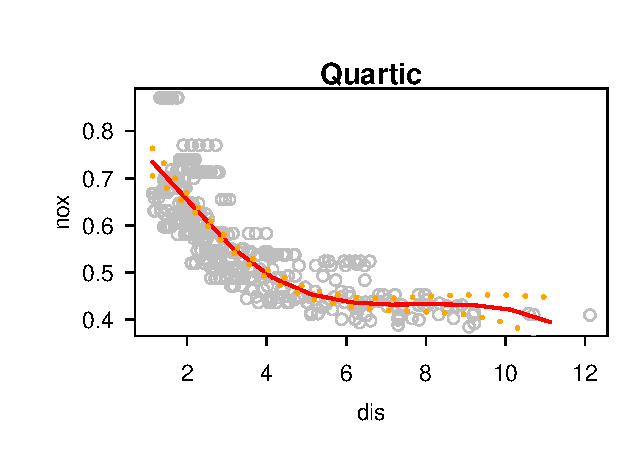
\includegraphics[width=.6\linewidth]{figure/Schmidt-HW7-Rnwunnamed-chunk-5-1} 

}


\begin{kframe}\begin{alltt}
\hlkwd{attr}\hlstd{(}\hlkwd{bs}\hlstd{(dis,} \hlkwc{df} \hlstd{=} \hlnum{4}\hlstd{),} \hlstr{"knots"}\hlstd{)}
\end{alltt}
\begin{verbatim}
##   50% 
## 3.207
\end{verbatim}
\end{kframe}
\end{knitrout}
\begin{knitrout}
\definecolor{shadecolor}{rgb}{0.969, 0.969, 0.969}\color{fgcolor}\begin{kframe}
\begin{alltt}
\hlcom{# Code for *Question E*}
\hlstd{RSS_reg_splines} \hlkwb{<-} \hlkwd{rep}\hlstd{(}\hlnum{NA}\hlstd{,} \hlnum{18}\hlstd{)}
\hlkwa{for} \hlstd{(i} \hlkwa{in} \hlnum{3}\hlopt{:}\hlnum{20}\hlstd{) \{}
    \hlstd{reg_spline_fit} \hlkwb{<-} \hlkwd{lm}\hlstd{(nox} \hlopt{~} \hlkwd{bs}\hlstd{(dis,} \hlkwc{df} \hlstd{= i),} \hlkwc{data} \hlstd{= Boston)}
    \hlstd{RSS_reg_splines[i]} \hlkwb{<-} \hlkwd{sum}\hlstd{(reg_spline_fit}\hlopt{$}\hlstd{residuals}\hlopt{^}\hlnum{2}\hlstd{)\}}
\hlkwd{par}\hlstd{(}\hlkwc{mfrow} \hlstd{=} \hlkwd{c}\hlstd{(}\hlnum{1}\hlstd{,}\hlnum{2}\hlstd{),} \hlkwc{mar} \hlstd{=} \hlkwd{c}\hlstd{(}\hlnum{4.5}\hlstd{,}\hlnum{4.5}\hlstd{,}\hlnum{1}\hlstd{,}\hlnum{1}\hlstd{),} \hlkwc{oma} \hlstd{=} \hlkwd{c}\hlstd{(}\hlnum{0}\hlstd{,}\hlnum{0}\hlstd{,}\hlnum{4}\hlstd{,}\hlnum{0}\hlstd{))}
\hlstd{RSS} \hlkwb{<-} \hlstd{RSS_reg_splines[}\hlopt{-}\hlkwd{c}\hlstd{(}\hlnum{1}\hlstd{,} \hlnum{2}\hlstd{)]}
\hlkwd{plot}\hlstd{(}\hlnum{1}\hlopt{:}\hlnum{18}\hlstd{, RSS,} \hlkwc{xlab} \hlstd{=} \hlstr{"Degrees"}\hlstd{,} \hlkwc{ylab} \hlstd{=} \hlstr{"Test RSS"}\hlstd{,} \hlkwc{type} \hlstd{=} \hlstr{"l"}\hlstd{)}
\hlstd{d.min} \hlkwb{<-} \hlkwd{which.min}\hlstd{(RSS);} \hlkwd{title}\hlstd{(}\hlstr{"Question E:  RSS"}\hlstd{,} \hlkwc{outer} \hlstd{=} \hlnum{FALSE}\hlstd{)}
\hlkwd{points}\hlstd{(}\hlkwd{which.min}\hlstd{(RSS), RSS[}\hlkwd{which.min}\hlstd{(RSS)],} \hlkwc{col} \hlstd{=} \hlstr{"red"}\hlstd{,} \hlkwc{cex} \hlstd{=} \hlnum{2}\hlstd{,} \hlkwc{pch} \hlstd{=} \hlnum{20}\hlstd{)}

\hlcom{# Code for *Question F*}
\hlstd{prediction_error} \hlkwb{<-} \hlkwd{rep}\hlstd{(}\hlnum{0}\hlstd{,} \hlnum{20}\hlstd{);} \hlkwd{set.seed}\hlstd{(}\hlnum{232}\hlstd{)}
\hlkwa{for} \hlstd{(i} \hlkwa{in} \hlnum{1}\hlopt{:}\hlnum{20}\hlstd{)\{} \hlcom{# Run all the polynomial models and store them}
  \hlcom{# Use the glm function for poly models instead of lm so we can use cv.glm}
   \hlstd{reg_spline_fit} \hlkwb{<-} \hlkwd{glm}\hlstd{(nox} \hlopt{~} \hlkwd{bs}\hlstd{(dis,} \hlkwc{df} \hlstd{= i),} \hlkwc{data} \hlstd{= Boston)}
   \hlstd{prediction_error[i]} \hlkwb{<-} \hlkwd{cv.glm}\hlstd{(Boston, reg_spline_fit,} \hlkwc{K} \hlstd{=} \hlnum{10}\hlstd{)}\hlopt{$}\hlstd{delta[}\hlnum{1}\hlstd{]\}}
\hlkwd{plot}\hlstd{(}\hlnum{1}\hlopt{:}\hlnum{20}\hlstd{, prediction_error,} \hlkwc{xlab} \hlstd{=} \hlstr{"Degree"}\hlstd{,} \hlkwc{ylab} \hlstd{=} \hlstr{"CV Error"}\hlstd{,} \hlkwc{type} \hlstd{=} \hlstr{"l"}\hlstd{)}
\hlstd{d.min} \hlkwb{<-} \hlkwd{which.min}\hlstd{(prediction_error);} \hlkwd{title}\hlstd{(}\hlstr{"Question F:  CV Error"}\hlstd{,} \hlkwc{outer} \hlstd{=} \hlnum{FALSE}\hlstd{)}
\hlkwd{points}\hlstd{(}\hlkwd{which.min}\hlstd{(prediction_error), prediction_error[}\hlkwd{which.min}\hlstd{(prediction_error)],}
       \hlkwc{col} \hlstd{=} \hlstr{"red"}\hlstd{,} \hlkwc{cex} \hlstd{=} \hlnum{2}\hlstd{,} \hlkwc{pch} \hlstd{=} \hlnum{20}\hlstd{)}
\end{alltt}
\end{kframe}

{\centering 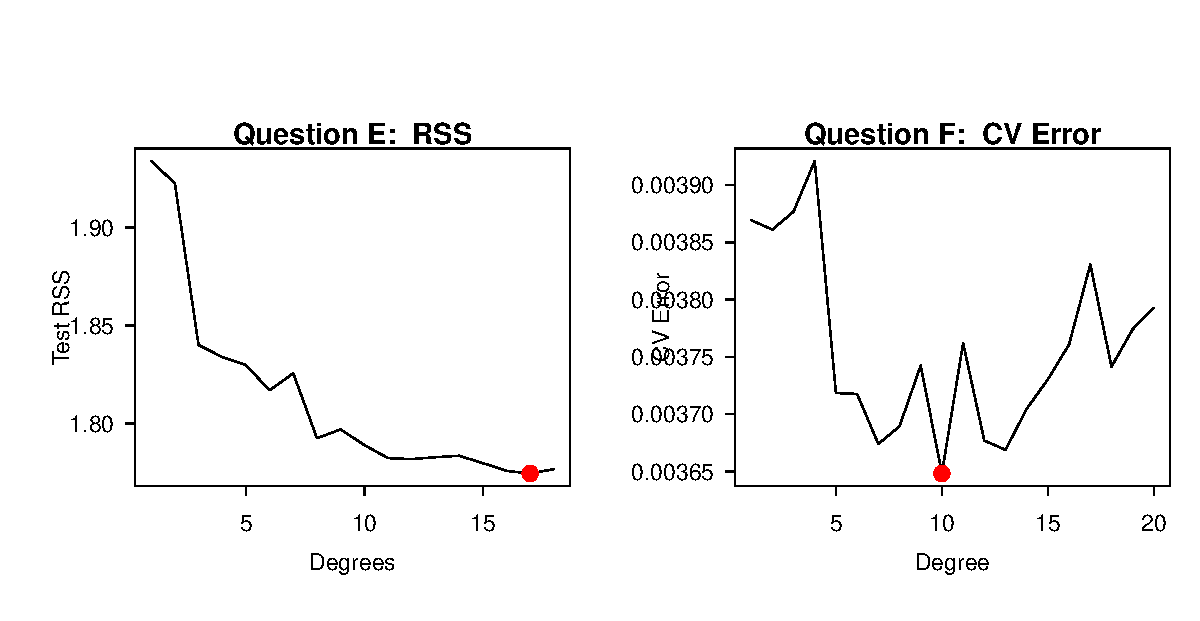
\includegraphics[width=.6\linewidth]{figure/Schmidt-HW7-Rnwunnamed-chunk-6-1} 

}



\end{knitrout}

The R session information (including the OS info, R version and all
packages used):

\begin{knitrout}
\definecolor{shadecolor}{rgb}{0.969, 0.969, 0.969}\color{fgcolor}\begin{kframe}
\begin{alltt}
\hlkwd{sessionInfo}\hlstd{()}
\end{alltt}
\begin{verbatim}
## R version 3.2.4 (2016-03-10)
## Platform: x86_64-apple-darwin13.4.0 (64-bit)
## Running under: OS X 10.9.5 (Mavericks)
## 
## locale:
## [1] en_US.UTF-8/en_US.UTF-8/en_US.UTF-8/C/en_US.UTF-8/en_US.UTF-8
## 
## attached base packages:
## [1] splines   stats     graphics  grDevices utils     datasets  methods   base     
## 
## other attached packages:
## [1] shiny_0.12.2 boot_1.3-18  MASS_7.3-45  ISLR_1.0     knitr_1.12.3
## 
## loaded via a namespace (and not attached):
##  [1] Rcpp_0.12.4       digest_0.6.9      mime_0.4          R6_2.1.1         
##  [5] jsonlite_0.9.17   xtable_1.7-4      formatR_1.3       magrittr_1.5     
##  [9] evaluate_0.8.3    highr_0.5.1       stringi_1.0-1     rstudioapi_0.3.1 
## [13] tools_3.2.4       stringr_1.0.0     markdown_0.7.7    httpuv_1.3.3     
## [17] rsconnect_0.4.1.4 htmltools_0.3.5
\end{verbatim}
\begin{alltt}
\hlkwd{Sys.time}\hlstd{()}
\end{alltt}
\begin{verbatim}
## [1] "2016-05-01 10:02:35 EDT"
\end{verbatim}
\end{kframe}
\end{knitrout}


\end{document}
